\section{Definicija derivacije}
\begin{definition}
Neka je $I\subseteq \mathbb{R}$ otvoreni interval. Kažemo da je $f : I\to \mathbb{R}$ \textbf{diferencijabilna} (ili \textit{derivabilna}) u točki $c\in I$ ako postoji $\lim\limits_{x\to c}{\dfrac{f(x)-f(c)}{x-c}}\in \mathbb{R}$. Taj broj zovemo \textbf{derivacija} funkcije $f$ u točki $c$ i označavamo ga s $f'(c)$. Nadalje, kažemo da je $f$ \textbf{diferencijabilna na $I$} ako je diferencijabilna u svakoj točki intervala $I$.
\end{definition}
Često se koristi i oznaka $\dfrac{\mathrm{d}f}{\mathrm{d}x}(c)$.

Ako je $I\subseteq \mathbb{R}$ otvoreni interval i $f : I\to \mathbb{R}$ diferencijabilna na $I$, onda funkciju $x\mapsto f'(x)$ zovemo \textbf{derivacija} funkcije $f$. Tako definiranu funkciju označavamo s $f'$, $\left(f(x)\right)'$, $\dfrac{\mathrm{d}f}{\mathrm{d}x}$, ili s $\dfrac{\mathrm{d}}{\mathrm{d}x}\left(f(x)\right)$.
\begin{remark}
Neka je $I\subseteq \mathbb{R}$ otvoreni interval. Tada je $f : I\to \mathbb{R}$ diferencijabilna u $c\in I$ ako i samo ako postoji $\lim\limits_{h\to 0}{\dfrac{f(c+h)-f(c)}{h}}$. Tada je
$$f'(c)=\lim\limits_{h\to 0}{\dfrac{f(c+h)-f(c)}{h}}.$$
\end{remark}
\begin{definition} Neka je $I\subseteq \mathbb{R}$ otvoreni interval i $c\in I$. Ako postoji limes $\lim\limits_ {x\to c+}{\dfrac{f(x)-f(c)}{x-c}}\in \mathbb{R}$, taj broj zovemo \textbf{desna derivacija} funkcije $f$ u točki $c$ i označavamo ga s $f_d'(c)$. Analogno, ako postoji limes $\lim\limits_ {x\to c-}{\dfrac{f(x)-f(c)}{x-c}}\in \mathbb{R}$, zovemo ga \textbf{lijeva derivacija} funkcije $f$ u točki $c$ i označavamo ga s $f_l'(c)$.
\end{definition}
\begin{exercise} \textbf{}
\label{firstder}
\begin{itemize}
\item[a)] Dokažite da je $x\mapsto x^3$ diferencijabilna na $\mathbb{R}$ i odredite joj derivaciju.
\item[b)] Je li $f : \mathbb{R}\to \mathbb{R}$,
$$f(x)=\begin{cases}
x^3, & x\geq 0,\\
x, & x\leq 0.
\end{cases}$$
diferencijabilna na $\mathbb{R}$?
\end{itemize}
\end{exercise}
\begin{proof}[Rješenje]
a) Neka je $c\in \mathbb{R}$ proizvoljan. Vrijedi
$$\lim\limits_{x\to c}{\dfrac{x^3-c^3}{x-c}}=\lim\limits_{x\to c}{\dfrac{(x-c)(x^2+xc+c^2)}{x-c}}=\lim\limits_{x\to c}{\left(x^2+xc+c^2\right)}=3c^2.$$
Dakle, za sve $c\in \mathbb{R}$, $x\mapsto x^3$ je diferencijabilna u $c$ i vrijedi $f'(c)=3c^2$. Stoga je derivacija funkcije $x\mapsto x^3$ funkcija $x\mapsto 3x^2$.

b) Tvrdimo da $f$ nije diferencijabilna u $0$. Zaista, vrijedi $$f_d'(0)=\lim\limits_{x\to 0+}{f'(x)}=\lim\limits_{x\to 0+}{\dfrac{x^3}{x}}=0,$$
a s druge strane imamo 
$$f_l'(0)=\lim\limits_{x\to 0-}{f'(x)}=\lim\limits_{x\to 0-}{\dfrac{x}{x}}=1,$$
dakle $f$ nije diferencijabilna na $\mathbb{R}$.
\end{proof}

\begin{exercise} \textbf{}
\begin{itemize}
\item[a)] Navedite primjer funkcije $f : \mathbb{R}\to \mathbb{R}$ takve da je $f'(1)=1$ i $f'(5)=2$.
\item[b)] Navedite primjer funkcije $f : \mathbb{R}\to \mathbb{R}$ koja je neprekidna na $\mathbb{R}$, te diferencijabilna svugdje osim u točkama $1$ i $2$.
\end{itemize}
\end{exercise}
\begin{proof*}
a) Znamo da je npr. za $a\in \mathbb{R}$, $\left(ax\right)'=a$, stoga možemo uzeti npr. $f : \mathbb{R}\to \mathbb{R}$,
$$f(x)=\begin{cases}
x, & x\leq 2,\\
5x, & x\geq 2.
\end{cases}$$
Primijetimo da je $f'(1)=1$. Zaista, očito vrijedi
\[
\pushQED{\qed}
\lim\limits_{x\to 1}{\dfrac{f(x)-f(1)}{x-1}}=\lim\limits_{x\to 1}{\dfrac{x-1}{x-1}}=1.\qedhere
\popQED
\]
\end{proof*}
\begin{remark}
Neka je $I\subseteq \mathbb{R}$ otvoreni interval i $f : I \to \mathbb{R}$ diferencijabilna u točki $c\in I$. Tada je $f$ i neprekidna u $c$.
\end{remark}
Obrat gornje napomene općenito ne vrijedi, i to npr. za funkciju $x\mapsto |x|$. Intuitivno, klasični primjeri funkcija koje su neprekidne ali ne i diferencijabilne u nekoj točki su one čiji grafovi imaju "šiljak" u toj točki.
\begin{exercise} \textbf{}
\label{idkhowtonamethis}
\begin{itemize}
\item[a)] Postoji li $c>0$ takav da je $f : \mathbb{R}\to \mathbb{R}$,
$$f(x)=\begin{cases}
cx^3,& x\geq 0,\\
-x^2-1-c,& x<0.
\end{cases}$$
diferencijabilna na $\mathbb{R}$?
\item[b)] Odredite sve $a, b\in \mathbb{R}$ takve da je $g : \mathbb{R}\to \mathbb{R}$,
$$g(x)=\begin{cases}
x^3,& x\leq 1,\\
ax+b,& x>1.
\end{cases}$$
diferencijabilna na $\mathbb{R}$.
\item[c)] Odredite neku funkciju $F : \langle -3, 3\rangle\to \mathbb{R}$ takvu da funkcija $c:\mathbb{R}\to \mathbb{R}$,
$$c(x)=\begin{cases}
-8,& x\leq -3,\\
F(x),& x\in \langle -3, 3\rangle,\\
8,& x\geq 3.
\end{cases}$$
bude diferencijabilna na $\mathbb{R}$.
\end{itemize}
\end{exercise}
\begin{proof}[Rješenje]
a) Pretpostavimo da postoji takav $c>0$. Da bi $f$ bila diferencijabilna u $0$, mora biti i neprekidna u $0$. Vrijedi
$$\lim\limits_{x\to 0+}{f(x)}=\lim\limits_{x\to 0+}{cx^3}=0,\;\; \lim\limits_{x\to 0-}{f(x)}=\lim\limits_{x\to 0-}{-x^2-1-c}=-1-c,$$
Kako je $-1-c<0$, lijevi i desni limes ne mogu biti jednaki, pa ne postoji takav $c$.

b) Slično kao i u a), uspoređivanjem lijevog i desnog limesa vidimo da mora vrijediti $a+b=1$. S druge strane, imamo $g_d'(1)=a$ i analogno $g_l'(1)=3$, stoga mora vrijediti $a=3$. Odavde imamo da je $b=-2$. Očito je za ovako odabrane $a$ i $b$ funkcija $g$ diferencijabilna u $1$. Ako je $x>1$, onda je $g'(x)=\dfrac{\mathrm{d}}{\mathrm{d}x}(ax+b)=a$, a za $x<1$ imamo $g'(x)=\dfrac{\mathrm{d}}{\mathrm{d}x}(x^3)=3x^2$. Stoga je $g$ diferencijabilna na $\mathbb{R}$ ako i samo ako je $a=3$ i $b=-2$.

c) Funkcija $f : \mathbb{R}\to \mathbb{R}$, $f(x)=x^3$ ima svojstvo $f'(0)=0$, pa će ideja biti njezin graf translatirati tako da točka ishodišta prijeđe u npr. točku $(-3, 8)$, tj. za $3$ jedinične dužine ulijevo i $8$ jediničnih dužina prema dolje (te ga, naravno, i restringirati tako da konačna funkcija $F$ ima domenu $\langle -3, 3\rangle$). Tražena funkcija je (v. napomenu \ref{graphrem}) $g : \langle -3, 1]\to \mathbb{R}$, 
$$g(x)=(x+3)^3-8,$$
(v. sliku \ref{dergraph}). Uočimo da je $g$ "na pola puta" između $-8$ i $8$ gledajući po $y$-osi upravo u svojoj nultočki, tj. točki $(-1,0)$, pa će sada biti ideja uzeti funkciju $h : [-1, 1]\to \mathbb{R}$ koja će biti pogodna translacija dijela "lijevog dijela" grafa funkcije $x\mapsto (x+3)^3-8$, tako da iz točke $(-1, 0)$ dođemo do točke $(1, 8)$, na način da vrijedi $h_d'(1)=0$. Uočimo da je $g'(-1)=12$, te je broj $a\in \mathbb{R}$, $a\neq -1$ takav da je $g'(a)=12$, broj $a=-5$, pa kako želimo da se desna derivacija od $g$ te lijeva derivacija od $h$ u točki $-1$ i njihove funkcijske vrijednosti u toj točki podudaraju, zahtijevati ćemo da točka $(-5, -16)$ prijeđe u točku $(-1, 0)$. Slijedi da graf funkcije $g$ moramo translatirati za $4$ jedinične dužine udesno i $16$ jediničnih dužina prema gore, čime dobivamo 
$$h(x)=(x-1)^3+8.$$ Sada je $h(1)=8$ i $h_d'(1)=0$, pa kako bi došli do točke $(3, 8)$ možemo iskoristiti dio grafa konstantne funkcije $x\mapsto 8$. Dakle, tražena funkcija biti će $F : \langle -3, 3\rangle\to \mathbb{R}$,
$$F(x)=\begin{cases}
(x+3)^3-8, & x\in \langle -3, -1],\\
(x-1)^3+8, & x\in [-1, 1],\\
8, & x\in [1, 3\rangle.
\end{cases}$$
Nije teško provjeriti da je $F$ zaista diferencijabilna na $\mathbb{R}$.
\begin{figure}[ht]
\begin{subfigure}[t]{.5\textwidth}
\centering
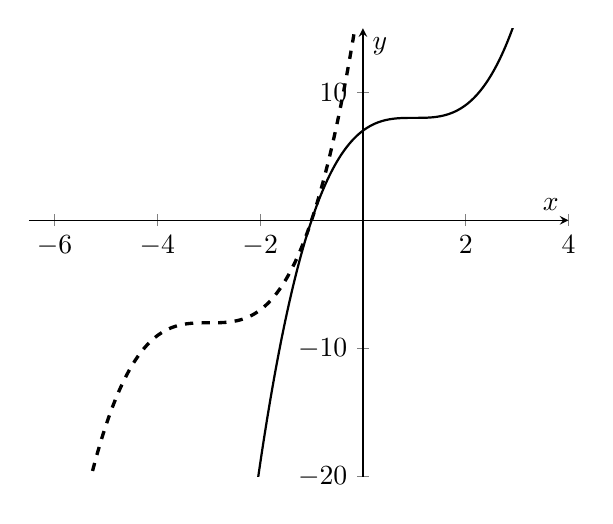
\begin{tikzpicture}
\begin{axis}[axis lines=middle,xlabel=$x$,ylabel=$y$,xmin=-6.5,xmax=4,ymin=-20,ymax=15, smooth, samples=200]

\addplot[very thick,dashed,color=black,domain=-8:1] {(x+3)^3-8};
\addplot[thick,color=black,domain=-3:3] {(x-1)^3+8};
\end{axis}
\end{tikzpicture}
\caption*{Grafovi funkcija $x\mapsto (x+3)^3-8$ (iscrtkana linija) i $x\mapsto (x-1)^3+8$ (puna linija)}
\end{subfigure}%
\begin{subfigure}[t]{.5\textwidth}
\centering
\begin{tikzpicture}
\begin{axis}[axis lines=middle,xlabel=$x$,ylabel=$y$,xmin=-6.5,xmax=4,ymin=-20,ymax=15, smooth, samples=200]

\addplot[thick,dotted,color=black,domain=-20:-3] {-8};
\addplot[very thick,dashed,color=black,domain=-3:-1] {(x+3)^3-8};
\addplot[thick,color=black,domain=-1:1] {(x-1)^3+8};
\addplot[very thick,dashdotted,color=black,domain=1:3] {8};
\addplot[thick,dotted,color=black,domain=3:4] {8};
\end{axis}
\end{tikzpicture}
\caption*{Graf funkcije $F$ iz rješenja c) dijela zadatka \ref{idkhowtonamethis}}
\end{subfigure}
\caption{\label{dergraph}}
\end{figure}
\end{proof}
\newpage
\begin{exercise}
Odredite sve točke u kojima je funkcija $f : \mathbb{R}\to \mathbb{R}$,
$$f(x)=\begin{cases}
x^3,& x\in \mathbb{Q},\\
x^4,& x\in \mathbb{I},
\end{cases}$$
diferencijabilna.
\end{exercise}
\begin{proof}[Rješenje]
Tvrdimo da je $f$ diferencijabilna samo u $0$. Zaista, za sve $x\in \mathbb{R}$ takve da je $|x|<1$ množenjem s $|x|^3$ dobivamo $x^4<|x|^3$, pa vrijedi
$$0\leq \left|\dfrac{f(x)}{x}\right|=\dfrac{|f(x)|}{|x|}\leq \dfrac{x^4}{|x|}=|x|^3,$$
pa kako $|x|^3\to 0$ kako $x\to 0$, iz kriterija sendviča za limese funkcija i iz činjenice da je pri promatranju limesa u $0$ dovoljno promatrati vrijednosti dovoljno "blizu" $0$, slijedi da postoji $\lim\limits_{x\to 0}{\left|\dfrac{f(x)}{x}\right|}=f'(0)$ i iz definicije limesa slijedi
$$0=\lim\limits_{x\to 0}{\left|\dfrac{f(x)}{x}\right|}=\lim\limits_{x\to 0}{\dfrac{f(x)}{x}}=f'(0).$$
Neka je sada $c=1$, te neka je $(a_n)$ niz racionalnih brojeva različitih od $1$ koji konvergira u $1$, te $(b_n)$ niz iracionalnih brojeva različitih od $1$ koji konvergira u $1$. Tada za sve $n\in \mathbb{N}$ vrijedi
$$\lim\limits_{n\to \infty}{\dfrac{f(a_n)-1}{a_n-1}}=\lim\limits_{n\to \infty}{\dfrac{a_n^3-1}{a_n-1}}=\lim\limits_{n\to \infty}{\dfrac{(a_n-1)\left(1+a_n+a_n^2\right)}{a_n-1}}=\lim\limits_{n\to \infty}{\left(1+a_n+a_n^2\right)}=3,$$
te se slično vidi i da je $\lim\limits_{n\to \infty}{\dfrac{f(b_n)-1}{b_n-1}}=4$, pa iz Heineove karakterizacije limesa slijedi da funkcija $x\mapsto \dfrac{f(x)-1}{x-1}$ nema limes u $1$, odnosno ne postoji $f'(1)$.

Neka je sada $c\notin \{0, 1\}$. Tvrdimo da tada $f$ nije neprekidna u točki $c$. Zaista, lako se provjeri da je $x^4=x^3$ ako i samo ako je $x=0$ ili $x=1$. Uzmimo sada niz $(x_n)$ racionalnih brojeva koji konvergira u $c$, te niz $(y_n)$ iracionalnih brojeva koji konvergira u $c$. Tada vrijedi $\lim\limits_{n\to \infty}{x_n^3}=c^3$ i $\lim\limits_{n\to \infty}{x_n^4}=c^4$, pa kako je $c^3\neq c^4$, iz Heineove karakterizacije neprekidnosti slijedi da $f$ nije neprekidna, pa ni diferencijabilna u $c$.
\end{proof}
\begin{exercise} 
\label{localder}
Neka je $I\subseteq \mathbb{R}$ otvoreni interval i $f : I \to \mathbb{R}$ diferencijabilna u $c\in I$. Dokažite da ako je $f'(c)>0$, da tada postoji $\delta>0$ takav da vrijedi
$$
\begin{cases}
x\in \langle c-\delta, c\rangle\cap I\Rightarrow f(x)<f(c),\\
x\in \langle c, c+\delta\rangle\cap I\Rightarrow f(x)>f(c).
\end{cases}
$$
\end{exercise}
\begin{proof}[Rješenje]
Po definiciji, za $\epsilon=f'(c)$ postoji $\delta>0$ takav da za sve $x\in I$ takve da je $0<|x-c|<\delta$ vrijedi
$$0<\dfrac{f(x)-f(c)}{x-c}<2f'(c)$$
Ako je $x>c$, tj. $x\in \langle c,c+\delta\rangle\cap I$, tada množenjem nejednakosti $0<\dfrac{f(x)-f(c)}{x-c}$ s $x-c$ dobivamo $f(x)>f(c)$. Analogno za $x<c$, odnosno $x\in \langle c-\delta, c\rangle\cap I$ dobivamo $f(x)<f(c)$.
\end{proof}

\begin{exercise}
Dokažite da je $x\mapsto \ln{x}$ diferencijabilna na $\langle 0,\infty\rangle$ i odredite joj derivaciju.
\end{exercise}
\begin{proof}[Rješenje]
Neka je $c>0$ proizvoljan. Imamo
$$\lim\limits_{x\to c}{\dfrac{\ln{x}-\ln{c}}{x-c}}=\lim\limits_{x\to c}{\dfrac{\ln{\dfrac{x}{c}}}{x-c}}=\lim\limits_{x\to c}{\ln\left(\left(\dfrac{x}{c}\right)^\frac{1}{x-c}\right)}.$$
Uočimo da vrijedi
$$\lim\limits_{x\to c}{\left(\dfrac{x}{c}\right)^\frac{1}{x-c}}=\lim\limits_{x\to c}{\left(\dfrac{x-c+c}{c}\right)^\frac{1}{x-c}}=\lim\limits_{x\to c}{\left(1+\dfrac{x-c}{c}\right)^\frac{1}{x-c}}=\lim\limits_{x\to c}{\left(\left(1+\dfrac{x-c}{c}\right)^\frac{c}{x-c}\right)^\frac{1}{c}}.$$
Želimo supstituirati $y=\dfrac{x-c}{c}$, pa se želimo uvjeriti da su zadovoljeni svi uvjeti teorema 13 u \cite{14}. Zaista, neka su $f, g : \langle 0, \infty\rangle\setminus\{c\}\to \mathbb{R}$ dane s 
$$f(x)=\left((1+x)^\frac{1}{x}\right)^\frac{1}{c},\;\;\;\;g(x)=\dfrac{x-c}{c}.$$ 
Tada je $f\circ g$ definirana na $\langle 0, \infty\rangle\setminus\{c\}$, $f$ ima limes $0$ u $c$ i $g$ ima limes u $e^\frac{1}{c}$ u $0$, te npr. za $\epsilon=c$ vrijedi da je $f(x)\neq 0$ za sve $x\in \langle c-\epsilon, c+\epsilon\rangle$, $x\neq c$, budući da je na tom intervalu $f$ strogo monotona. Stoga je
$$\lim\limits_{x\to c}{\left(\dfrac{x}{c}\right)^\frac{1}{x-c}}=\lim\limits_{x\to c}{\left(\left(1+\dfrac{x-c}{c}\right)^\frac{c}{x-c}\right)^\frac{1}{c}}=\lim\limits_{y\to 0}{\left((1+y)^\frac{1}{y}\right)^\frac{1}{c}}=e^\frac{1}{c}.$$
Odavde i iz činjenice da je $\ln$ neprekidna u $c$ $\left(\text{pa ima limes u }f(c)\right)$ i strogo rastuća, analognom primjenom teorema 13 u \cite{14} slijedi
$$\lim\limits_{x\to c}{\ln\left(\left(\dfrac{x}{c}\right)^\frac{1}{x-c}\right)}=\ln{e^\frac{1}{c}}=\dfrac{1}{c}.$$
Stoga je $\ln$ diferencijabilna na $\langle 0, \infty\rangle$ i njezina derivacija je $x\mapsto \dfrac{1}{x}$.
\end{proof}
\begin{exercise}
Neka je $I\subseteq \mathbb{R}$ otvoreni interval i $f : I \to \mathbb{R}$ diferencijabilna na $I$. Koristeći do sada poznate rezultate, dokažite da ako za sve $x\in I$ vrijedi $f'(x)\geq 0$, da je tada $f$ rastuća.
\end{exercise}
\begin{proof}[Rješenje]
Pretpostavimo suprotno, tj. da postoje $x_1, x_2\in I$ takvi da je $x_1<x_2$, ali $f(x_1)>f(x_2)$. Ideja dokaza će biti sljedeća -- u segmentu $[x_1, x_2]$ ćemo promotriti najveći element za koji $f$ postiže maksimum na tom segmentu. Najprije ćemo dokazati da taj najveći element uopće postoji i to tako da ga definiramo kao supremum svih elemenata koji postižu maksimum na segmentu. Svaki element u segmentu strogo veći od tog elementa će dakle biti strogo manji od tog elementa, što će biti u kontradikciji sa zadatkom \ref{localder}.

Neka je 
$$S=\left\{x\in [x_1, x_2] : f(x)=\max{f|_{[x_1, x_2]}}\right\}.$$ 
Uočimo da je $f$ neprekidna na segmentu $[x_1, x_2]$ i na tom segmentu nije konstanta, pa postoji bar jedan $x_i\in [x_1, x_2]$ takav da je $f(x_i)=\max{f|_{[x_1, x_2]}}$. Dakle, postoji $\sup{S}$.

Tvrdimo da je $\sup{S}\neq x_2$. Zaista, po zadatku \ref{localder} postoji $\delta>0$ takav da za sve $x\in \langle x_2-\delta, x_2\rangle\cap I$ vrijedi $f(x)<f(x_2)$. S druge strane, po lemi \ref{14} imamo da za $\epsilon=\delta$ postoji $x_0\in [x_1, x_2]$ takav da je $f(x_0)=\max{f|_{[x_1, x_2]}}$ i vrijedi $x_2-\delta<x_0$. Pritom vrijedi $x_0<x_2$, jer kad bi bilo $x_0=x_2$, onda bi vrijedilo $f(x_2)=\max{f|_{[x_1, x_2]}}$, što je kontradikcija s činjenicom da je $f(x_2)<f(x_1)$. Sada iz činjenice da je $x_0\in \langle x_2-\delta, x_2\rangle\cap I$ slijedi da je $f(x_0)<f(x_2)$, što je kontradikcija s činjenicom da je $f(x_0)=\max{f|_{[x_1, x_2]}}$.

Kako je $S\subseteq [x_1, x_2]$, to je $\sup{S}\leq \sup{[x_1, x_2]}=x_2$, pa iz činjenice da je $\sup{S}\neq x_2$ imamo da je $\sup{S}<x_2$. Dokažimo i da je
$\sup{S}=\max{S}.$
Zaista, po lemi \ref{14} za svaki $n\in \mathbb{N}$ postoji $z_n\in [x_1, x_2]$ takav da je $f(z_n)=\max{f|_{[x_1, x_2]}}$ i vrijedi $\sup{S}-\dfrac{1}{n}<z_n$. Promotrimo niz $(z_n)$. Očito vrijedi $z_n\leq \sup{S}$, pa po kriteriju sendviča imamo $\lim\limits_{x\to\infty}{z_n}=\sup{S}$, pa iz činjenice da je $f$ diferencijabilna, pa i neprekidna u $\sup{S}$ slijedi
$$f(\sup{S})=\lim\limits_{x\to\infty}{f(z_n)}=\lim\limits_{x\to\infty}{\max{f|_{[x_1, x_2]}}}=\max{f|_{[x_1, x_2]}}.$$
Odavde imamo da je $\sup{S}\in S$, pa je i $\sup{S}=\max{S}$.

Konačno, kako je $f'(\max{S})>0$, postoji $\delta>0$ takav da za sve $x\in \langle \max{S}, \max{S}+\delta\rangle\cap I$ vrijedi $f(x)>f(\max{S})$. Neka je $\delta'=\min\{\delta, x_2-\max{S}\}$. Tada je 
$$\max{S}+\delta'\leq \max{S}+x_2-\max{S}=x_2,$$
pa za sve $\langle \max{S}, \max{S}+\delta'\rangle\cap I\subseteq \langle \max{S}, x_2\rangle$ vrijedi $f(x)>f(\max{S})$. No ovo znači da npr. vrijedi $$f\left(\max{S}+\dfrac{\delta'}{2}\right)>f(\max{S}).$$ S druge strane, kako je $\max{S}+\dfrac{\delta'}{2}\in [x_1, x_2]$ i $\max{S}+\dfrac{\delta'}{2}>\max{S}$, vrijedi $\max{S}+\dfrac{\delta'}{2}\notin S$,
pa je $f\left(\max{S}+\dfrac{\delta'}{2}\right)<\max{f|_{[x_1, x_2]}}=f(\max{S})$, kontradikcija!
\end{proof}
\section{Osnovne operacije s diferencijabilnim funkcijama}
\begin{remark}[Osnovne operacije s diferencijabilnim funkcijama]
Neka je $I\subseteq \mathbb{R}$ otvoreni interval, te $f, g : I\to \mathbb{R}$ diferencijabilne u točki $c\in I$. Tada vrijede sljedeće tvrdnje.
\begin{itemize}
\item[a)] Funkcija $f+g$ je diferencijabilna u $c$ i vrijedi $(f+g)'(c)=f'(c)+g'(c)$,
\item[b)] Funkcija $fg$ je diferencijabilna u $c$ i vrijedi $(fg)'(c)=f'(c)g(c)+f(c)g'(c)$,
\item[c)] Ako je $a\in \mathbb{R}$, onda je $af$ diferencijabilna u $c$ i vrijedi $(af)'(c)=a\cdot f'(c)$.
\item[d)] Ako je $g(c)\neq 0$, onda je $\left(\dfrac{f}{g}\right)$ diferencijabilna u $c$ i vrijedi $$\left(\dfrac{f}{g}\right)'(c)=\dfrac{f'(c)g(c)-f(c)g'(c)}{g(c)^2}.$$ 
\end{itemize}
\end{remark}
\begin{remark}[Derivacije elementarnih funkcija] Sljedeće tvrdnje vrijede za sve $x$ iz prirodne domene pripadnih funkcija.
\begin{AutoMultiColItemize}
\item $(c)'=0$, gdje je $c\in \mathbb{R}$
\item $(x^a)'=ax^{a-1}$, gdje je $a\in\mathbb{R}$ i $x\neq 0$ ako je $a<1$,
\item $(\sin{x})'=\cos{x}$,
\item $(\cos{x})'=-\sin{x}$,
\item $(\tg{x})'=\dfrac{1}{\cos^2{x}}$,
\item $(\ctg{x})'=-\dfrac{1}{\sin^2{x}}$,
\item $(a^x)'=a^x\ln{a}$, gdje je $a>0$
\item $(e^x)'=e^x$,
\item $(\arcsin{x})'=\dfrac{1}{\sqrt{1-x^2}}$,
\item $(\arccos{x})'=-\dfrac{1}{\sqrt{1-x^2}}$,
\item $(\arctg{x})'=\dfrac{1}{1+x^2}$,
\item $(\arcctg{x})'=-\dfrac{1}{1+x^2}$,
\item $(\log_a{x})'=\dfrac{1}{x\ln{a}}$, gdje je $a>0, a\neq 1$,
\item $(\ln{x})'=\dfrac{1}{x}$,
\item $(\sh{x})'=\ch{x}$,
\item $(\ch{x})'=\sh{x}$,
\item $(\th{x})'=\dfrac{1}{\ch^2{x}}$,
\item $(\cth{x})'=-\dfrac{1}{\sh^2{x}}$,
\item $(\arsinh{x})'=\dfrac{1}{\sqrt{1+x^2}}$,
\item $(\arcosh{x})'=\dfrac{1}{\sqrt{x^2-1}}$,
\item $(\artanh{x})'=\dfrac{1}{1-x^2}$,
\item $(\arcoth{x})'=\dfrac{1}{1-x^2}$
\end{AutoMultiColItemize}
\end{remark}
\begin{exercise} \textbf{}
\begin{itemize}
\item[a)] Dokažite da je funkcija $x\mapsto x^3\sin{x}+\sqrt{x}\ln{x}$ diferencijabilna na $\langle 0,\infty\rangle$ i odredite joj derivaciju.
\item[b)] Dokažite da je funkcija $x\mapsto e^x\cdot\sh{x}\cdot\arctg{x}$ diferencijabilna na $\mathbb{R}$ i odredite joj derivaciju.
\end{itemize}
\end{exercise}
\begin{proof}[Rješenje]
a) Neka je $c>0$ proizvoljan. Uočimo da je svaka od funkcija $x\mapsto \sin{x}$, $x\mapsto x^3$, $x\mapsto \sqrt{x}$, $x\mapsto \ln{x}$ diferencijabilna na $\langle 0,\infty\rangle$, pa i u $c$, pa slijedi i da su funkcije $x\mapsto x^3\sin{x}$ i $x\mapsto \sqrt{x}\ln{x}$ diferencijabilne u $c$, te posljedično je i funkcija iz iskaza zadatka diferencijabilna u $c$, odakle slijedi diferencijabilnost na $\langle 0,\infty\rangle$. Vrijedi
\begin{align*}
\left(x^3\sin{x}+\sqrt{x}\ln{x}\right)'&=\left(x^3\sin{x}\right)'+\left(\sqrt{x}\ln{x}\right)'\\
&=3x^2\sin{x}+x^3\cos{x}+\dfrac{1}{2\sqrt{x}}\ln{x}+\dfrac{\sqrt{x}}{x},
\end{align*}
gdje $\left(\sqrt{x}\right)'=\dfrac{1}{2\sqrt{x}}$ slijedi iz činjenice da je $\left(\sqrt{x}\right)'=\left(x^\frac{1}{2}\right)'=\dfrac{1}{2}x^{\frac{1}{2}-1}=\dfrac{1}{2}x^{-\frac{1}{2}}=\dfrac{1}{2\sqrt{x}}$.

b) $x\mapsto e^x\cdot \sh{x}$ i $x\mapsto \arctg{x}$ su diferencijabilne na $\mathbb{R}$, pa je i funkcija iz zadatka diferencijabilna na $\mathbb{R}$. Vrijedi
\begin{align*}
\left(e^x\cdot\sh{x}\cdot\arctg{x}\right)'&=\left(e^x\cdot\sh{x}\right)'\arctg{x}+\left(e^x\cdot\sh{x}\right)\cdot \dfrac{1}{1+x^2}\\
&=\left(e^x\cdot \sh{x}+e^x\cdot \ch{x}\right)\arctg{x}+\left(e^x\cdot\sh{x}\right)\cdot \dfrac{1}{1+x^2}.\qedhere
\end{align*}
\end{proof}
\begin{remark}[Derivacija kompozicije funkcija]
Neka su $I, J\subseteq \mathbb{R}$ otvoreni intervali, $c\in I$, te $f : I\to \mathbb{R}$, $g : J\to \mathbb{R}$ funkcije takve da je $f(I)\subseteq J$. Ako je $f$ diferencijabilna u $c$ i $g$ diferencijabilna u $f(c)$, onda je i $g\circ f$ diferencijabilna u $c$ i vrijedi
$$\left(g\circ f\right)'(c)=g'\left(f(c)\right)\cdot f'(c).$$
\end{remark}
\begin{remark}[Teorem o derivaciji inverzne funkcije]
Neka je $I\subseteq \mathbb{R}$ otvoreni interval, $c\in I$, $f : I\to \mathbb{R}$ strogo monotona na $I$, te $J=f(I)$ otvoreni interval. Ako je $f$ diferencijabilna u $c$ i vrijedi $f'(c)\neq 0$, tada je $f^{-1}$ diferencijabilna u $d=f(c)$ i vrijedi
$$\left(f^{-1}\right)\left(f(c)\right)=\dfrac{1}{f'(c)}=\dfrac{1}{f'\left(f^{-1}(d)\right)}.$$
\end{remark}
\begin{exercise} \textbf{}
\begin{itemize}
\item[a)] Dokažite da je funkcija $x\mapsto \sqrt{x^2+4x+5}$ diferencijabilna na $\mathbb{R}$ i odredite joj derivaciju.
\item[b)] Odredite derivaciju funkcije $x\mapsto \sqrt{x^2+\sin(\ln{x})}$ na intervalu $\langle 1,\infty\rangle$.
\item[c)] Zadana je $y : \left\langle -\dfrac{\pi}{4}, \dfrac{\pi}{4}\right\rangle\to \mathbb{R}$, $y(x)=2\tg{2x}$. Vrijedi li $y'(x)-y^2(x)=4$ za sve $x\in \left\langle -\dfrac{\pi}{4}, \dfrac{\pi}{4}\right\rangle$?
\end{itemize}
\end{exercise}
\newpage
\begin{proof}
a) Prvo uočimo da je $x^2+4x+5>0$ za sve $x\in \mathbb{R}$, jer je vodeći koeficijent jednak $1$ i diskriminanta jednaka $16-20=-4<0$\footnote{Općenito, ako su $a, b, c\in \mathbb{R}$ takvi da je $a>0$ i $b^2-4ac<0$, onda je $ax^2+bx+c>0$ za sve $x\in \mathbb{R}$. Zaista, za sve $x\in \mathbb{R}$ vrijedi $ax^2+bx+c\geq \dfrac{4ac-b^2}{4a}>0$. Intuicija iza te činjenice je da je zbog $a>0$ parabola koja je graf funkcije $x\mapsto ax^2+bx+c$ okrenuta "prema gore" i zbog negativne diskriminante nema nultočki.}. Nadalje, neka je $c\in \mathbb{R}$. Tada je $x\mapsto x^2+4x+5$ diferencijabilna u $c$, $x\mapsto \sqrt{x}$ diferencijabilna u $c^2+4c+5$, pa je i funkcija iz zadatka diferencijabilna u $c$, dakle na $\mathbb{R}$. Vrijedi
$$\left(\sqrt{x^2+4x+5}\right)'=\dfrac{1}{2\sqrt{x^2+4x+5}}\cdot\left(2x+4\right).$$

b) U narednim zadatcima nećemo provjeravati diferencijabilnost, jer se to radi potpuno analogno kao u prethodnim zadatcima. Vrijedi
\begin{align*}
\left(\sqrt{x^2+\sin(\ln{x})}\right)'&=\dfrac{1}{2\sqrt{x^2+\sin(\ln{x})}}\cdot \left(x^2+\sin\left(\ln{x}\right)\right)'\\
&=\dfrac{1}{2\sqrt{x^2+\sin(\ln{x})}}\cdot \left(2x+\cos\left(\ln{x}\right)\cdot\dfrac{1}{x}\right).
\end{align*}

c) Neka je $x\in \left\langle -\dfrac{\pi}{4}, \dfrac{\pi}{4}\right\rangle$. Vrijedi
$$\left(2\tg{2x}\right)'-4\tg^2{2x}=2\cdot\dfrac{1}{\cos^2{2x}}\cdot 2-4\tg^2{2x}=4\cdot \left(\dfrac{1}{\cos^2{2x}}-\tg^2{2x}\right)=4,$$
gdje posljednja jednakost iz činjenice da za sve $y\in \mathbb{R}$ takve da je $\cos^2{y}\neq 0$ vrijedi $$\tg^2{y}+1=\dfrac{1}{\cos^2{y}},$$
što se dobiva iz identiteta $\sin^2{y}+\cos^2{y}=1$ dijeljenjem obje strane s $\cos^2{y}$.
\end{proof}
\begin{exercise}
Dokažite da je funkcija $f : \mathbb{R}\to \mathbb{R}$,
$$f(x)=\begin{cases}
\arctg\left(3\sin{x}\right),& x\leq 0,\\
\sin{x}+2x\cos{x},& x>0.
\end{cases}$$
Dokažite da je $f$ diferencijabilna u $0$.
\end{exercise}
\begin{proof}[Rješenje]
Ideja će biti promatrati funkcije $f_1, f_2 : \mathbb{R}\to \mathbb{R}$, $f_1(x)=\arctg\left(3\sin{x}\right)$, $f_2(x)=\sin{x}+2x\cos{x}$, te dovesti u vezu derivacije tih funkcija u $0$ s $f_l'(0)$ i $f_d'(0)$. Zaista, dovoljno je pokazati da je $f_1(0)=f_2(0)=0$ i da postoje $f_l'(0)$ i $f_d'(0)$ te da vrijedi $f_l'(0)=f_d'(0)$. Zaista, u tom slučaju postoji $f'(0)$, jer je
$$f_1'(0)=\lim\limits_{x\to 0}{\dfrac{f_1(x)-f_1(0)}{x-0}}=\lim\limits_{x\to 0^-}{\dfrac{f_1(x)}{x}}=\lim\limits_{x\to 0^-}{\dfrac{f(x)}{x}}=f_l'(0)$$
i analogno $f_2'(0)=f_d'(x)$. Odavde po karakterizaciji limesa funkcije pomoću jednostranih limesa slijedi egzistencija od $f'(0)$. 

Očigledno je $f_1(0)=f_2(0)=0$. Uočimo da vrijedi
\begin{align*}
\left(\arctg\left(3\sin{x}\right)\right)'&=\dfrac{1}{1+\left(3\sin{x}\right)^2}\cdot \left(3\cos{x}\right),\\
\left(\sin{x}+2x\cos{x}\right)'&=\cos{x}+2\cos{x}-2x\sin{x}=3\cos{x}-2x\sin{x},
\end{align*}
pa je $f_1'(0)=f_2'(0)=3$, što je i trebalo pokazati.
\end{proof}
\begin{exercise}
Zadana je funkcija $f : \mathbb{R}\to \mathbb{R}$, $f(x)=2e^x+1$. Odredite derivaciju funkcije $f^{-1}$ koristeći teorem o derivaciji inverzne funkcije i direktno iz formule za inverznu funkciju.
\end{exercise}
\begin{proof}[Rješenje]
Neka su $f_1, f_2 : \mathbb{R}\to \mathbb{R}$ dane sa $f_1(x)=e^x$, $f_2(x)=2x+1$. Uočimo da je $f=f_2\circ f_1$, odakle slijedi da je $f$ strogo rastuća (jer su $f_1$ i $f_2$ strogo rastuće) i $f(\mathbb{R})=f_2\left(f_1\left(\mathbb{R}\right)\right)=f_2\left(\langle 0, \infty\rangle\right)=\langle 1,\infty\rangle$. Za sve $x\in \mathbb{R}$ vrijedi $\left(2e^x+1\right)'=2e^x>0$, tj. $f'(x)\neq 0$. Neka je $d\in \langle 1, \infty\rangle$. Tada postoji $c\in \mathbb{R}$ takav da je $f(c)=d$, odnosno $c=f^{-1}(d)$. Vrijedi
\begin{align}
\label{invderexercise1}
\left(f^{-1}\right)'(d)=\dfrac{1}{f'\left(f^{-1}(d)\right)}=\dfrac{1}{2e^{f^{-1}(d)}}.
\end{align}
Ovime smo dobili formulu za $\left(f^{-1}\right)'$. Sada uočimo da za sve $y>1$ vrijedi
$$f^{-1}(y)=f_1^{-1}\left(f_2^{-1}\left(y\right)\right)=\ln{\dfrac{y-1}{2}},$$
te imamo
$$\left(f^{-1}\right)'(y)=\left(\ln{\dfrac{y-1}{2}}\right)'=\dfrac{2}{y-1}\cdot \dfrac{1}{2}=\dfrac{1}{y-1}.$$
Usporedimo sada ovo s (\ref{invderexercise1}). Za sve $y>1$ vrijedi
$$\dfrac{1}{2e^{\ln{\frac{y-1}{2}}}}=\dfrac{1}{2\cdot \dfrac{y-1}{2}}=\dfrac{1}{y-1},$$
odakle vidimo da dobivamo isto rješenje na oba načina.
\end{proof}
\begin{exercise}[Derivacija Lambertove W funkcije]
Neka je zadana $f : \langle -1, \infty\rangle\to \mathbb{R}$, $f(x)=xe^x$. Odredite derivaciju funkcije $f^{-1}$.
\end{exercise}
\begin{proof}[Rješenje]
Može se pokazati da vrijedi $\mathcal{R}(f)=\left\langle-\dfrac{1}{e}, \infty\right\rangle$ i da je $f$ strogo rastuća, pa je dobro definirana funkcija $f^{-1} : \left\langle-\dfrac{1}{e}, \infty\right\rangle\to \mathbb{R}$. Neka je sada $z>-1$ proizvoljan. Uočimo da je $f$ diferencijabilna u svakoj točki $x\in \mathbb{R}$ i vrijedi
$$\left(xe^x\right)'=e^x+xe^x,$$
pa kako je $x\mapsto e^x+xe^x$ strogo rastuća na $\langle -1, \infty\rangle$ (kao zbroj strogo rastućih funkcija na tom intervalu), za sve $x, y\in \langle -1, \infty\rangle$ takve da je $x<y<z$ vrijedi $f'(x)<f'(y)<f'(z)$. Funkcija $f'$ ima limes slijeva jednak $0$ u točki $-1$, te funkcija $x\mapsto f'(y)$ ima limes zdesna jednak $f'(y)$, pa vrijedi 
$$0=\lim\limits_{x\to -1^+}{f'(x)}\leq f'(y),$$
što znači da vrijedi $f'(z)>f'(y)\geq 0$, odnosno $f'(z)>0$, pa kako je $z$ bio proizvoljan, vrijedi $f'(z)\neq 0$ za sve $z\in \langle -1,\infty\rangle$.

Neka je sada $d\in \left\langle-\dfrac{1}{e}, \infty\right\rangle$. Tada postoji $c\in \langle -1,\infty\rangle$ takav da je $d=f(c)$, tj. takav da je $f^{-1}(d)=c$. Očito je $f$ diferencijabilna u $c$ i vrijedi $f'(c)\neq 0$, pa imamo
$$\left(f^{-1}\right)'(d)=\dfrac{1}{f'\left(f^{-1}(d)\right)}=\dfrac{1}{e^{f^{-1}(d)}+f^{-1}(d)\cdot e^{f^{-1}(d)}}=\dfrac{1}{d+e^{f^{-1}(d)}},$$
gdje posljednja jednakost slijedi iz svojstava inverzne funkcije.
\end{proof}
\begin{exercise}
Dokažite teorem o derivaciji inverzne funkcije.
\end{exercise}
\begin{proof}[Rješenje]
Želimo se uvjeriti da vrijedi
$$\lim\limits_{y\to d}{\dfrac{f^{-1}(y)-f^{-1}(d)}{y-d}}=\dfrac{1}{f'(c)},$$
što možemo pokazati tako da dokažemo da je funkcija $i : J\to \mathbb{R}$ dana sa
$$i(y)=\begin{cases}
\dfrac{f^{-1}(y)-f^{-1}(d)}{y-d}, & y\neq f(c),\\
\dfrac{1}{f'(c)}, & y=f(c).
\end{cases}$$
neprekidna u $f(c)$, što možemo pokazati na način da je u točki $f(c)$ prikažemo kao kompoziciju neprekidnih funkcija.
Promotrimo funkciju $h : I\to \mathbb{R}$ danu sa
$$h(x)=\begin{cases}
\dfrac{f(x)-f(c)}{x-c}, & x\neq c,\\
f'(c), & x=c.
\end{cases}$$
Kako je $f$ diferencijabilna u $c$, slijedi i da je $h$ neprekidna u $c$. No tada je i $\dfrac{1}{h}$ neprekidna u $c$ i vrijedi
\begin{align}
\label{invproof}
\left(\dfrac{1}{h}\right)(x)=\dfrac{1}{h(x)}=\begin{cases}
\dfrac{x-c}{f(x)-f(c)}, & x\neq c,\\
\dfrac{1}{f'(c)}, & x=c.
\end{cases}
\end{align}
Po teoremu o neprekidnosti inverzne funkcije je također i $f^{-1}$ neprekidna u $d=f(c)$, pa je stoga $\dfrac{1}{h}\circ f^{-1}$ neprekidna u $f(c)$ i za sve $y\in J$ vrijedi
$$\left(\dfrac{1}{h}\circ f^{-1}\right)(y)=i(y)=\dfrac{1}{h\left(f^{-1}(y)\right)}=\begin{cases}
\dfrac{f^{-1}(y)-f^{-1}(d)}{y-d}, & y\neq f(c),\\
\dfrac{1}{f'(c)}, & y=f(c).
\end{cases}$$
Zaista, ako je $y=f(c)$, onda je $f^{-1}(y)=c$, pa tvrdnja slijedi iz (\ref{invproof}), a ako je $y\neq f(c)$, onda je i $f^{-1}(y)\neq c$ (kontrapozicija dane tvrdnje glasi da iz $f^{-1}(y)=c$ slijedi $y=f(c)$ što očito vrijedi jer je $f$ funkcija). Odavde slijedi tvrdnja teorema.
\end{proof}
U sljedećem zadatku dokazujemo da je tangenta u točki $c$ na graf diferencijabilne funkcije od svih pravaca "najbolja" aproksimacija te funkcije blizu točke $c$.
\begin{exercise}
Neka je $I$ otvoreni interval, $c\in I$, $a, b\in \mathbb{R}$, te $f : I \to \mathbb{R}$ diferencijabilna na $I$. Neka su $g, h : \mathbb{R}\to \mathbb{R}$ dane s $g(x)=f'(c)(x-c)+f(c)$, $h(x)=ax+b$\footnote{Obratite pozornost na to da ovdje može biti $a=0$.}. Tada postoji $\delta_h>0$ takav da za sve $x\in I$ vrijedi
$$0<|x-c|<\delta_h\Rightarrow |f(x)-g(x)|<|f(x)-h(x)|.$$
\end{exercise}

% Dodati zadatak gdje se neka vrijednost aproksimira linearnom funkcijom